\documentclass[aspectratio=169,11pt]{beamer}
\usepackage{presentation-theme}
\hypersetup{pdftitle={Does periodic teacher promotion improve chemical semantics?},pdfauthor={Wuhao},pdfsubject={Checkpoint audit, 29 September 2026}}
\newcommand{\MaeAUC}{0.824}
\newcommand{\PromotedAUC}{0.814}
\newcommand{\InitialAUC}{0.834}
\newcommand{\LatestAUC}{0.814}
\newcommand{\MaccsDelta}{-0.020}
\newcommand{\RepeatCount}{2,659}
\newcommand{\RandomTanimoto}{0.095}
\newcommand{\MassTanimoto}{0.115}
\newcommand{\PermutationAUC}{0.497}

\newcommand{\bodytext}[4]{\node[anchor=north west,inner sep=0,align=left,text width=#3cm,font=\figurefont\fontsize{10}{13}\selectfont] at (#1,#2) {#4};}
\newcommand{\plotfigure}[1]{\node[anchor=north,inner sep=0] at (8,6.78) {\includegraphics[width=14.3cm,height=4.75cm,keepaspectratio]{figures/#1_slide.pdf}};}
\newcommand{\freshsource}{Fresh audit: MassSpecGym 1.5; 22,746 / 3,185 / 2,998 train / validation / test molecules. One centroid per InChIKey; frozen encoders.}
\newcommand{\oldsource}{Reanalyzed 28 Sep results: 194,119 / 19,429 / 17,556 spectra; spectrum weighting. These are supporting, exploratory comparisons.}
\begin{document}

\begin{frame}
\begin{tikzpicture}[remember picture,overlay,shift={(current page.south west)}]
\header{REPRESENTATION AUDIT / 29 SEP 2026}{}
\node[anchor=north west,inner sep=0,font=\brandmedium\fontsize{25}{29}\selectfont,text width=13.8cm,align=left] at (.75,7.25) {Does promoting the student\\make chemistry emerge?};
\bodytext{.85}{5.0}{13.8}{\textbf{A tradeoff, not a general improvement.}\\Global similarity and peak-dropout robustness improve. Chemical readouts, local neighbors and repeat-spectrum retrieval worsen.}
\bodytext{.85}{3.48}{8.3}{Initial teacher \(\rightarrow\) 24 promotions \(\rightarrow\) step 1,209,000\\A fresh audit plus existing depth and attention probes}
\node[anchor=north west,inner sep=0,font=\brandmedium\fontsize{25}{28}\selectfont] at (10.3,3.5) {\MaccsDelta};
\bodytext{10.3}{2.55}{4.5}{Change in final-mean\\MACCS AUROC}
\takeaway{The evidence does not support automatic semantic improvement from promotion.}
\source{Three exact encoder states; one training run. No matched never-promoted control: the causal contribution of promotion remains unidentified.}
\end{tikzpicture}
\end{frame}

\begin{frame}
\begin{tikzpicture}[remember picture,overlay,shift={(current page.south west)}]
\header{01 / DEFINE THE CLAIM}{Three meanings of ``semantic structure''}
\foreach \x/\title in {1.05/Information,6.0/Geometry,11.0/Robustness}{\node[anchor=north west,inner sep=0,font=\brandmedium\fontsize{16}{18}\selectfont] at (\x,6.35) {\title};}
\bodytext{1.05}{5.35}{3.9}{Can a frozen embedding predict chemical fingerprints and properties?}
\bodytext{6.0}{5.35}{3.9}{Do nearby embeddings correspond to chemically similar molecules?}
\bodytext{11.0}{5.35}{3.9}{Does the same molecule remain recognizable across spectral variation?}
\draw[line] (5.35,3.05)--(5.35,6.5);\draw[line] (10.35,3.05)--(10.35,6.5);
\bodytext{1.05}{3.15}{3.9}{Chemical probes\\Label efficiency}
\bodytext{6.0}{3.15}{3.9}{Chemical neighbors\\Similarity correlations}
\bodytext{11.0}{3.15}{3.9}{Measured repeats\\Controlled perturbations}
\takeaway{A strong trained readout alone does not establish a useful native distance metric.}
\source{Operational definitions for this investigation. ``Natural'' geometry is tested with raw cosine; transformations are separate sensitivity analyses.}
\end{tikzpicture}
\end{frame}

\begin{frame}
\begin{tikzpicture}[remember picture,overlay,shift={(current page.south west)}]
\header{02 / LINEAGE}{The initial teacher already learned chemistry}
\diagramblock{3.05}{5.4}{3.9}{1.1}{MAE ancestor\\step 666,000}
\diagramblock{8.0}{5.4}{3.9}{1.1}{Frozen-teacher JEPA\\step 1,190,000}
\draw[arr] (5.05,5.4)--(5.98,5.4);
\node[tag] at (5.55,5.97) {supervises};
\bodytext{10.6}{5.93}{4.4}{This JEPA student becomes\\the \textbf{initial teacher}.}
\draw[arr] (8,4.8)--(8,4.0);
\diagramblock{3.05}{3.35}{3.9}{.9}{Fresh periodic student\\random initialization}
\diagramblock{8.0}{3.35}{3.9}{.9}{Promote every 50,000\\completed updates}
\draw[arr] (5.05,3.35)--(5.98,3.35);
\bodytext{10.6}{3.95}{4.3}{\textbf{24 promotions}\\Teacher: 1,200,000\\Student: 1,209,000}
\takeaway{Compare to the JEPA initial teacher, not only to a random encoder or the MAE ancestor.}
\source{Verified W\&B config, GCS checkpoint listing and promotion implementation. Latest saved: 1,209,000; W\&B last logged: 1,208,750; run state: crashed.}
\end{tikzpicture}
\end{frame}

\begin{frame}
\begin{tikzpicture}[remember picture,overlay,shift={(current page.south west)}]
\header{03 / OPTIMIZATION}{Lower prediction loss is not a semantic guarantee}
\plotfigure{training_loss}
\takeaway{Promotion changes the target function; losses across generations are not a fixed semantic yardstick.}
\source{Actual W\&B telemetry: 4,835 non-null training points and 120 validation points. Dashed lines indicate scheduled teacher-copy steps, not extra observations.}
\end{tikzpicture}
\end{frame}

\begin{frame}
\begin{tikzpicture}[remember picture,overlay,shift={(current page.south west)}]
\header{04 / SUPPORTING DEPTH SWEEP}{The initial teacher is stronger through much of the encoder}
\plotfigure{legacy_depth}
\takeaway{Learned encoders beat random features; the periodic endpoint does not improve the overall depth profile.}
\source{\oldsource\ Depth 0: embedder; 1--25: block outputs; final: output norm. Ridge penalties selected on validation. Layer comparisons are exploratory.}
\end{tikzpicture}
\end{frame}

\begin{frame}
\begin{tikzpicture}[remember picture,overlay,shift={(current page.south west)}]
\header{05 / FRESH CHEMICAL PROBES}{Balancing by molecule preserves the main finding}
\plotfigure{chemical_probes}
\takeaway{Final-mean MACCS AUROC: initial \InitialAUC\; versus latest \LatestAUC.}
\source{\freshsource\ Train-only standardization; eight ridge penalties selected on validation. 166 MACCS bits, 15 functional groups, seven properties. Undefined AUROCs excluded.}
\end{tikzpicture}
\end{frame}

\begin{frame}
\begin{tikzpicture}[remember picture,overlay,shift={(current page.south west)}]
\header{06 / NATIVE AND TRANSFORMED GEOMETRY}{Test chemical neighborhoods directly}
\plotfigure{geometry}
\takeaway{Raw cosine is the native test; centering, scaling and whitening probe how coordinate choice changes it.}
\source{\freshsource\ Morgan radius 2, 4,096 bits. Partial Spearman controls spectral cosine and precursor-mass gap; average ranks for ties. All transforms fitted on train only.}
\end{tikzpicture}
\end{frame}

\begin{frame}
\begin{tikzpicture}[remember picture,overlay,shift={(current page.south west)}]
\header{07 / UNCERTAINTY}{The main losses are larger than molecule-sampling noise}
\plotfigure{paired_uncertainty}
\takeaway{Paired comparisons reuse the same test molecules and preserve teacher--student pairing.}
\source{95\% percentile bootstrap intervals: 500 molecule resamples for macro AUROC, 2,000 for neighbor Tanimoto. Fixed trained models; no training-seed uncertainty or multiple-testing correction.}
\end{tikzpicture}
\end{frame}

\begin{frame}
\begin{tikzpicture}[remember picture,overlay,shift={(current page.south west)}]
\header{08 / REPRESENTATION SHAPE}{Mean geometry spreads; CLS becomes nearly one-dimensional}
\plotfigure{covariance}
\takeaway{Mean effective rank rises from 28 to 79; CLS puts 97.2\% of its variance in one component.}
\source{Covariance of train-molecule centroids. Effective rank: exp(entropy of normalized eigenvalues); PC1: largest variance fraction. Mean cosine includes self pairs (O(1/N) contribution).}
\end{tikzpicture}
\end{frame}

\begin{frame}
\begin{tikzpicture}[remember picture,overlay,shift={(current page.south west)}]
\header{09 / POSITIVE EVIDENCE}{Global chemical ordering improves despite weaker local neighbors}
\plotfigure{cls_exception}
\takeaway{Raw-mean partial Spearman rises from 0.153 to 0.243; the geometry result is mixed.}
\source{\freshsource\ 99,955 sampled distinct-molecule pairs; raw and train-standardized cosine are distinguished. Pairs share molecules; no pair-based confidence intervals.}
\end{tikzpicture}
\end{frame}

\begin{frame}
\begin{tikzpicture}[remember picture,overlay,shift={(current page.south west)}]
\header{10 / LABEL EFFICIENCY}{Check whether fewer labels unlock a new advantage}
\plotfigure{label_efficiency}
\takeaway{The same fixed encoder is probed with 1\%, 10\% and 100\% of training-molecule labels.}
\source{227 / 2,274 / 22,746 training molecules; deterministic subsamples. Each fraction fits its own train-only scaling and validation-selected ridge penalty. One subsample seed per fraction.}
\end{tikzpicture}
\end{frame}

\begin{frame}
\begin{tikzpicture}[remember picture,overlay,shift={(current page.south west)}]
\header{11 / CHEMICAL DETAIL}{Disaggregate the property readouts}
\plotfigure{properties}
\takeaway{Semantics are multidimensional: inspect individual chemistry targets as well as aggregate scores.}
\source{\freshsource\ Seven RDKit targets; one ridge penalty chosen by mean validation R². These are prediction scores, not chemical-generation or candidate-retrieval accuracies.}
\end{tikzpicture}
\end{frame}

\begin{frame}
\begin{tikzpicture}[remember picture,overlay,shift={(current page.south west)}]
\header{12 / ROBUSTNESS}{Stability is useful, but it is a separate objective}
\plotfigure{robustness}
\takeaway{Peak-dropout retrieval: 32\% to 99\%; metadata-zero retrieval: 95\% to 20\%; repeat retrieval: 36\% to 26\%.}
\source{Perturbations: one spectrum from each of 2,048 test molecules; fixed seed. Repeat retrieval: \RepeatCount\ molecules, two distinct rows each. Synthetic interventions, not validated physical acquisition models.}
\end{tikzpicture}
\end{frame}

\begin{frame}
\begin{tikzpicture}[remember picture,overlay,shift={(current page.south west)}]
\header{13 / STRONGER READOUTS}{Existing attention probes do not reverse the endpoint ordering}
\plotfigure{attentive}
\takeaway{Learning how to pool tokens does not reveal a hidden general advantage for the periodic student here.}
\source{\oldsource\ Two readout seeds; marks show both observations, lines show their mean. Epoch selected on validation MACCS AUROC; 12-epoch cap. Mean-linear includes CLS in its token mean.}
\end{tikzpicture}
\end{frame}

\begin{frame}
\begin{tikzpicture}[remember picture,overlay,shift={(current page.south west)}]
\header{14 / WHY THE HYPOTHESIS IS NOT A THEOREM}{Promotion supplies a new teacher, not a chemical objective}
\eqn[15]{1.0}{6.45}{\mathcal L=\mathbb E\,\|p(f_S(x_C),q_T)-\mathrm{sg}[f_T(x)_T]\|^2}
\bodytext{1.05}{5.23}{13.6}{For a fixed target and an unconstrained squared-error predictor, the optimal prediction is the \textbf{conditional mean of the target code} given the available input.}
\eqn[14]{1.0}{4.03}{p^*(u)=\mathbb E[z_T\mid u],\qquad \theta_T\leftarrow\theta_S\quad\text{every 50k updates}}
\bodytext{1.05}{3.15}{13.6}{Predictability can favor chemistry, but it can also favor mass, acquisition cues or an impoverished code. A constant student/teacher code is a possible zero-loss fixed point of the unconstrained formulation.}
\takeaway{Masking, retained variation and the training dynamics determine which predictable structure survives.}
\source{Conditional-mean statement assumes a fixed target distribution and unrestricted predictor; not a convergence theorem for this run. Related design evidence: Assran et al., I-JEPA (2023); Bardes et al., VICReg (2022).}
\end{tikzpicture}
\end{frame}

\begin{frame}
\begin{tikzpicture}[remember picture,overlay,shift={(current page.south west)}]
\header{15 / WHAT WE CAN CONCLUDE}{Evidence against the strong claim; no isolated causal estimate}
\bodytext{1.0}{6.45}{6.3}{\textbf{Observed}\\[6pt]Chemical signal above simple baselines.\\[6pt]Most endpoint chemical readouts worsen.\\[6pt]Some pooling and robustness measures differ.\\[6pt]Latest promoted teacher and student are close.}
\draw[line] (7.75,2.65)--(7.75,6.55);
\bodytext{8.25}{6.45}{6.7}{\textbf{Not established}\\[6pt]Promotion alone caused the deterioration.\\[6pt]Every generation gets worse.\\[6pt]The same result holds across seeds or masks.\\[6pt]Pretraining molecules never overlap this benchmark.}
\takeaway{For this checkpoint: retained chemistry, but no broad semantic improvement over its initial teacher.}
\source{Only one periodic-training seed; late checkpoints plus the initial teacher. Published benchmark folds are used, but pretraining overlap and structural split provenance were not independently reconstructed.}
\end{tikzpicture}
\end{frame}

\begin{frame}
\begin{tikzpicture}[remember picture,overlay,shift={(current page.south west)}]
\header{16 / NEXT DECISIVE EXPERIMENT}{Change the promotion rule while matching everything else}
\bodytext{1.0}{6.45}{13.7}{\textbf{Same initial teacher, same fresh student seeds, same batches and masks, same optimizer and token budget.}}
\diagramblock{3.05}{4.8}{3.7}{1.0}{Never promote\\fixed initial teacher}
\diagramblock{8.0}{4.8}{3.7}{1.0}{Promote every 50k\\current recipe}
\diagramblock{12.9}{4.8}{3.7}{1.0}{Slower promotion\\or EMA comparison}
\bodytext{1.0}{3.62}{13.7}{At least three matched seeds. Save each pre/post-promotion teacher and student. Track raw chemical neighbors, held-out probes, variance and acquisition dependence throughout training.}
\takeaway{Treat this as a proposed causal experiment, not a result already measured.}
\source{Use validation metrics for design selection and a new untouched test set for confirmation. Regularization and masking changes require separate, explicitly controlled arms.}
\end{tikzpicture}
\end{frame}

\begin{frame}
\begin{tikzpicture}[remember picture,overlay,shift={(current page.south west)}]
\header{APPENDIX / PROTOCOL}{What was run, and what was reused}
\bodytext{1.0}{6.5}{6.5}{\textbf{Fresh, 29 September}\\[5pt]Three states; all 231,104 spectra.\\[5pt]Block 13 / 19 / final mean and final CLS.\\[5pt]Probes, geometry, covariance, robustness and single-spectrum neighbors.\\[5pt]Paired bootstrap; shuffled-label control.}
\bodytext{8.15}{6.5}{6.7}{\textbf{Reanalyzed, 28 September}\\[5pt]27 depths \(\times\) mean / CLS.\\[5pt]Random and MAE reference encoders.\\[5pt]Two-seed attention and linear probes.\\[5pt]Legacy tie handling and test-fitted pairwise scaling limit these comparisons.}
\takeaway{Fresh metrics use a distinct, stricter protocol; do not subtract scores across protocols.}
\source{Original training remains JAX. Frozen evaluation reuses staged PyTorch encoder exports; state-conversion and promotion tests passed. Cached export hashes and source hashes are saved.}
\end{tikzpicture}
\end{frame}

\begin{frame}
\begin{tikzpicture}[remember picture,overlay,shift={(current page.south west)}]
\header{APPENDIX / SINGLE SPECTRUM}{The local-neighbor loss is not an averaging artifact}
\plotfigure{single_spectrum}
\takeaway{With one measured spectrum per molecule, raw neighbor Tanimoto falls from 0.173 to 0.161.}
\source{First file row per molecule: 22,746 train candidates, 2,998 test queries. Final valid-peak mean; no centroid averaging. Physical precursor window: ±5 Th, after undoing input normalization.}
\end{tikzpicture}
\end{frame}

\begin{frame}
\begin{tikzpicture}[remember picture,overlay,shift={(current page.south west)}]
\header{APPENDIX / CONTROLS AND LIMITS}{Useful negative controls, with realistic limits}
\bodytext{1.0}{6.4}{13.5}{\textbf{Fresh controls}\\Random training molecule: \RandomTanimoto\ Tanimoto. Nearest mean precursor mass: \MassTanimoto.\\Shuffled training labels: final-mean MACCS AUROC \PermutationAUC\ (initial teacher).}
\bodytext{1.0}{4.75}{13.5}{\textbf{Evaluation unit}\\Centroids average spectra sharing a full InChIKey. This uses identity labels for balancing; the separate single-spectrum check does not average spectra.}
\bodytext{1.0}{3.05}{13.5}{\textbf{Evidence scope}\\One dataset and one pretraining seed. Internal-layer and secondary outcomes are exploratory. No exact molecular-structure recovery claim.}
\takeaway{Confidence intervals describe molecule sampling, not all sources of experimental uncertainty.}
\source{Raw results, per-molecule predictions, checkpoint/config/data hashes, scripts, figure sources and the full W\&B snapshot accompany the report.}
\end{tikzpicture}
\end{frame}

\begin{frame}
\begin{tikzpicture}[remember picture,overlay,shift={(current page.south west)}]
\header{APPENDIX / REFERENCES}{Sources and reproducibility}
\bodytext{1.0}{6.4}{13.8}{\href{https://wandb.ai/iclac/jepa-finalrun/runs/1p8b-ptjepa-t1190k-p50k-b1024-v6e32-20260922-062250}{Periodic-teacher W\&B run} and saved GCS checkpoint metadata\\[8pt]\texttt{scripts/modal\_periodic\_semantics.py} --- fresh frozen-encoder audit\\\texttt{scripts/analyze\_periodic\_semantics.py} --- paired uncertainty\\\texttt{research/summary.json} --- full results\\[8pt]\href{https://arxiv.org/abs/2301.08243}{Assran et al. (2023), I-JEPA}: masking and predictive representations.\\\href{https://arxiv.org/abs/2105.04906}{Bardes et al. (2022), VICReg}: explicit control of variance and covariance.\\\href{https://arxiv.org/abs/2104.14294}{Caron et al. (2021), DINO}: empirical emergent semantics in a different recipe.}
\takeaway{The conclusions come from checkpoint measurements; the papers supply context, not proof for this run.}
\source{Built from repository sources with the existing virtual environment. See periodic\_semantics\_README.md for commands, caveats and the artifact inventory.}
\end{tikzpicture}
\end{frame}

\end{document}
